\documentclass[12pt,a4paper]{article}

\usepackage[utf8]{inputenc}
\usepackage[spanish]{babel}
\usepackage{listings}
\usepackage{graphicx}


\lstset{
  language=SQL,
  basicstyle=\ttfamily\small,
  keywordstyle=\bfseries,
  commentstyle=\itshape,
  frame=single,
  breaklines=true,
  showstringspaces=false,
  tabsize=4,
  numbers=left,
  numberstyle=\tiny,
  numbersep=8pt,
  captionpos=b,
}

\title{Análisis de ingeniería inversa sobre un sistema \textit{Legacy}}
\author{Luis Augusto Rojas Guerra}
\date{\today}

\begin{document}

\maketitle
\tableofcontents
\newpage

\section{Descripción general}

La base de datos \textbf{escuela} modela el sistema académico de una
institución educativa. Contempla la gestión de departamentos,
profesores, cursos, estudiantes, inscripciones, aulas, horarios y
calificaciones, interrelacionados mediante claves foráneas que
garantizan la integridad referencial.

\subsection{Resumen de tablas}

\begin{center}
\begin{tabular}{llc}
  \hline
  \textbf{Tabla} & \textbf{Descripción} & \textbf{Columnas} \\
  \hline
  \texttt{departamentos} & Áreas académicas de la institución   & 2 \\
  \texttt{profesores}    & Docentes asignados a un departamento       & 5 \\
  \texttt{cursos}        & Materias impartidas por un profesor        & 4 \\
  \texttt{estudiantes}   & Alumnos registrados en el sistema          & 5 \\
  \texttt{inscripciones} & Relación entre estudiantes y cursos      & 4 \\
  \texttt{aulas}         & Espacios físicos disponibles             & 3 \\
  \texttt{horarios}      & Programación de cursos en aulas          & 6 \\
  \texttt{notas}         & Calificaciones de cada inscripción       & 3 \\
  \hline
\end{tabular}
\end{center}

\section{Inicialización de la base de datos}

El bloque siguiente crea la base de datos si no existe y la selecciona
como contexto activo para todas las sentencias SQL posteriores.

\begin{lstlisting}[caption={Creación y selección de la base de datos}]
CREATE DATABASE IF NOT EXISTS escuela;
USE escuela;
\end{lstlisting}

\section{Definición de tablas}

\subsection{Tabla \texttt{departamentos}}

Almacena las áreas o facultades académicas a las que pertenecen los
profesores. Es la entidad raíz de la jerarquía organizativa.

\begin{center}
\begin{tabular}{llll}
  \hline
  \textbf{Columna} & \textbf{Tipo} & \textbf{Restricción} & \textbf{Descripción} \\
  \hline
  \texttt{id}     & \texttt{INT}          & PK, AUTO\_INCREMENT, NOT NULL & Identificador único \\
  \texttt{nombre} & \texttt{VARCHAR(100)} & NOT NULL                      & Nombre del departamento \\
  \hline
\end{tabular}
\end{center}

\begin{lstlisting}[caption={SQL -- departamentos}]
CREATE TABLE departamentos (
    id INT PRIMARY KEY AUTO_INCREMENT,
    nombre VARCHAR(100) NOT NULL
);
\end{lstlisting}

\section{Script completo de creación}

\lstinputlisting{escuela.sql}{Script SQL completo - base de datos escuela}

\section{Diagrama Entidad-Relación}

\begin{figure}[htbp]
    \centering 
    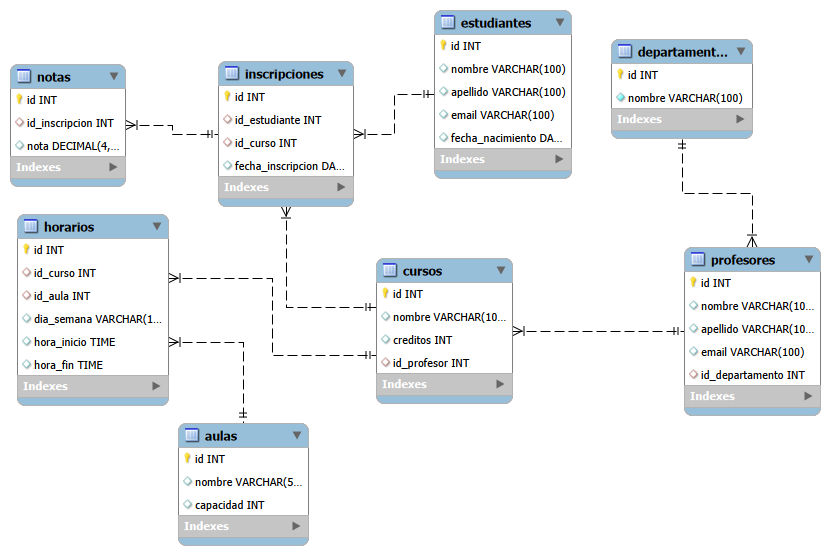
\includegraphics[width=0.8\textwidth]{./imgs/database}
    \caption{Diagrama EER - base de datos \textbf{escuela}}
\end{figure}

\end{document}